\section{Introduction}
\label{sec:Introduction}

%\subsection{Word Embeddings}

When neural networks process image or audio-data they usually work with rich, high-dimensional datasets.
For image data these might be vectors of individual pixel-intensities or for audio data vectors of power spectral density coefficients.
Natural language processing systems traditionally treat words as atomic symbols which are
encoded as simple indexes. For example 'apple' might become index $Id123$ and 'orange' becomes index $Id124$. This way the
encoding of the word data is arbitrary and contains no meaningful information regarding the relationships between word-symbols anymore.
In contrast to the dense representation of audio and image data, this way of encoding leads to data sparsity. Which means there is more data
required to sufficiently train our statistical models.

\begin{figure}[H]
\begin{center}
  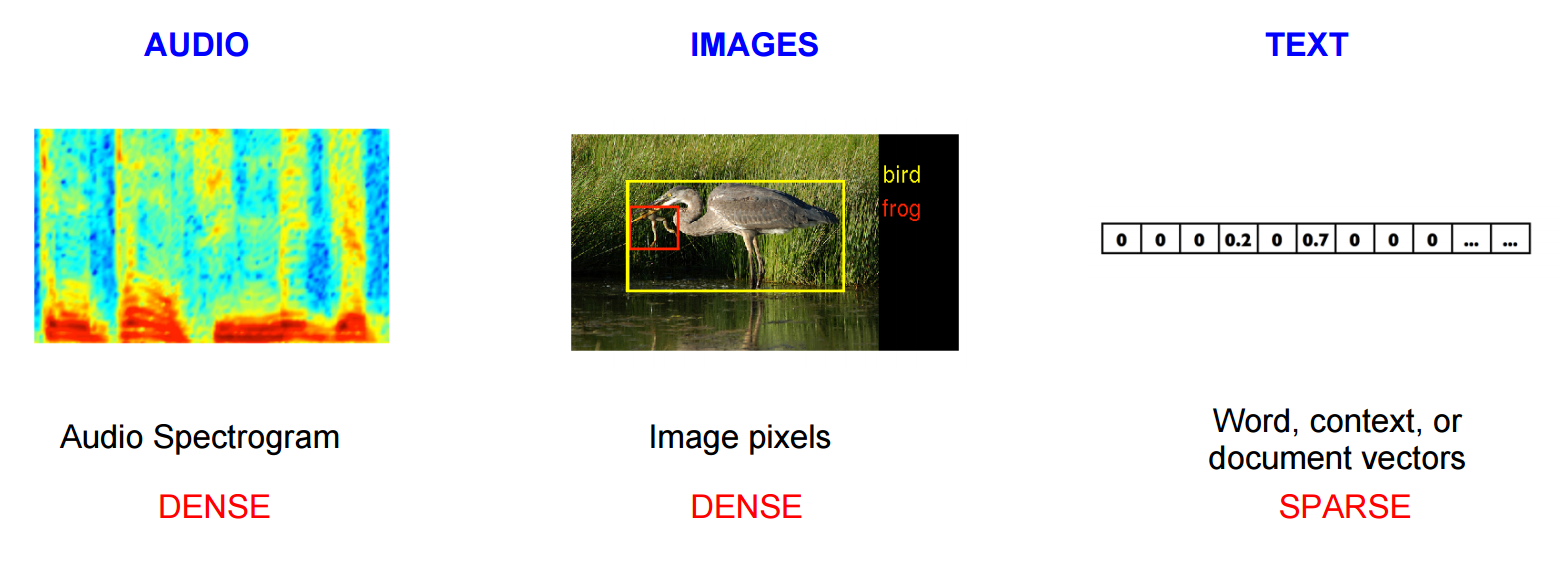
\includegraphics[width=\textwidth]{./img/audio-image-text}
  \caption{Comparison between the input datasets for different kinds of data (From~\cite{tensorflow:word2vec}).}
  \label{fig:audio-image-text}
\end{center}
\end{figure}

A statistical model can learn the relationships between word symbols (for example between 'apple' and 'apples') and leverage it for it's tasks.
Essentially we need to have a function which can take a word from the vocabulary and turn it into a feature vector.
The vectors are all in the same continuous vector space, in which we can now represent (embed) all words.
Ideally these feature vectors have a low dimension compared to the size of the vocabulary. Additionally words which have a
similar meaning (semantically similar) should be mapped to (geometrically) nearby points in the vector space.
They capture the intuitive understanding that words may be different 
or similar along a variety of dimensions in a quantifiable way.
An example can be seen in figure~\ref{fig:linear-relationships}, where some of these learned vectors representations
capture a semantic relationship between different words.

These vector representations of words are called "word embeddings" and a natural language processing 
system can use different methods to generate them.
All of these methods are based on the assumption that words which share semantic meaning tend to occur in the same contexts;
this is called the "Distributional Hypothesis"~\cite{Sahlgren2008}. 

\begin{figure}[H]
\begin{center}
  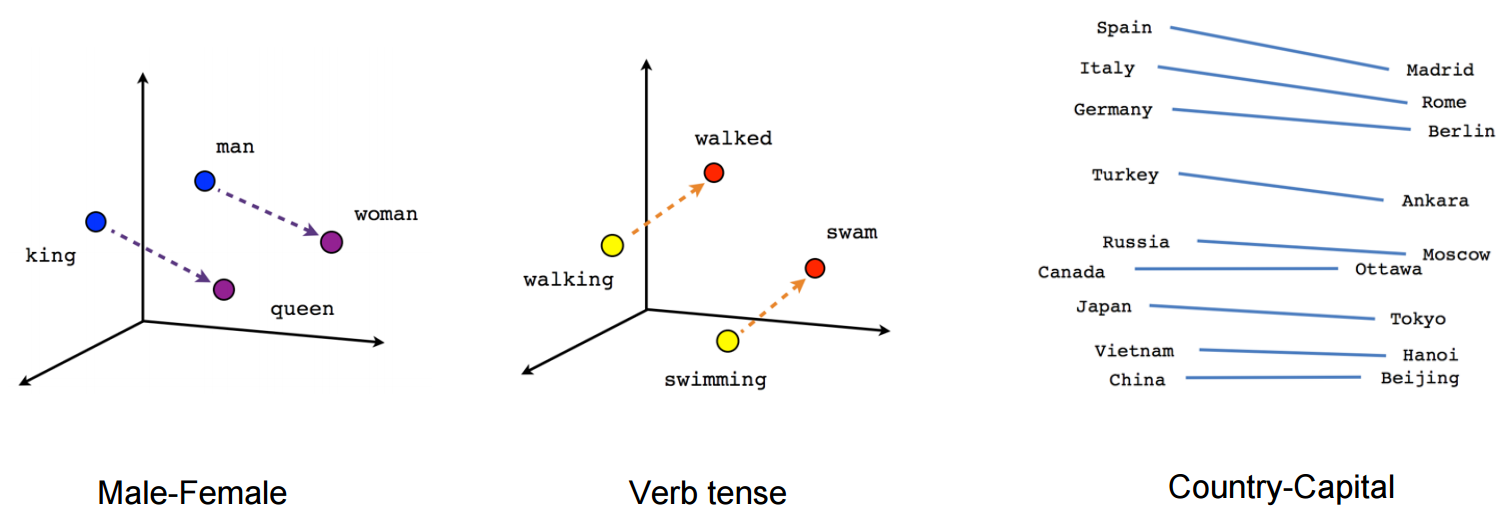
\includegraphics[width=\textwidth]{./img/linear-relationships}
  \caption{Visualization of word embeddings computed with the Skip-Gram model~\cite{DBLP:journals/corr/MikolovSCCD13}. 
  Vectors are projected onto 2 dimensions (Figure taken from~\cite{tensorflow:word2vec}).}
  \label{fig:linear-relationships}
\end{center}
\end{figure}

Formally we have our vocabulary $V$ and a function $f: V \rightarrow \mathbb{R}^d$ which maps $w \in V$ to a feature vector $\vec(w)$. 
A counting based approach to generate $f$ would be to perform a dimensionality reduction 
on a word co-occurrence matrix~\cite{DBLP:journals/corr/LebretL13}. The rows would then serve as the vectors.

However in this work we focus on recurrent neural networks to generate word embeddings. 
For example we will use the ability of neural nets to predict a word from the context (its neighbours) in which it appears. 
The first RNN will learn the vector embeddings as part of the larger processing system, 
in this case a natural network-based language model (NNLM).
By serving as the projection layer of the language model, the word embedding system is trained alongside with the rest of the model. 


% Many task's in Natural Language Processing (NLP) benefit from having a dense real-valued input vector, a good 
% embedding will improve outcomes for a lot of other tasks, like Part-of-Speech Tagging or language modeling.

% \subsection{Morphology}
% \label{subsec:Morphology}

% Short intro into morphology and why this is relevant to word embeddings.



% Text mit \"a, \"o, \"U, Stra{"s}e, Caf\'e.\\[4ex]
